\section{问题思考}

\begin{frame}{问题思考}
    \begin{itemize}
        \item 影像集: 遥感影像与其他图像区别
        \item 数据集: 真实数据与生成数据对比
        \item 模型: 不同模型超分效果对比
    \end{itemize}
\end{frame}

\subsection{影像集}
\begin{frame}{影像集}
    以realESRGAN模型为例, 分别使用预训练和finetune后的模型进行对比

    \begin{figure}[!htbp]
        \centering
        \subfloat[finetune]{\label{fig:0201a}
        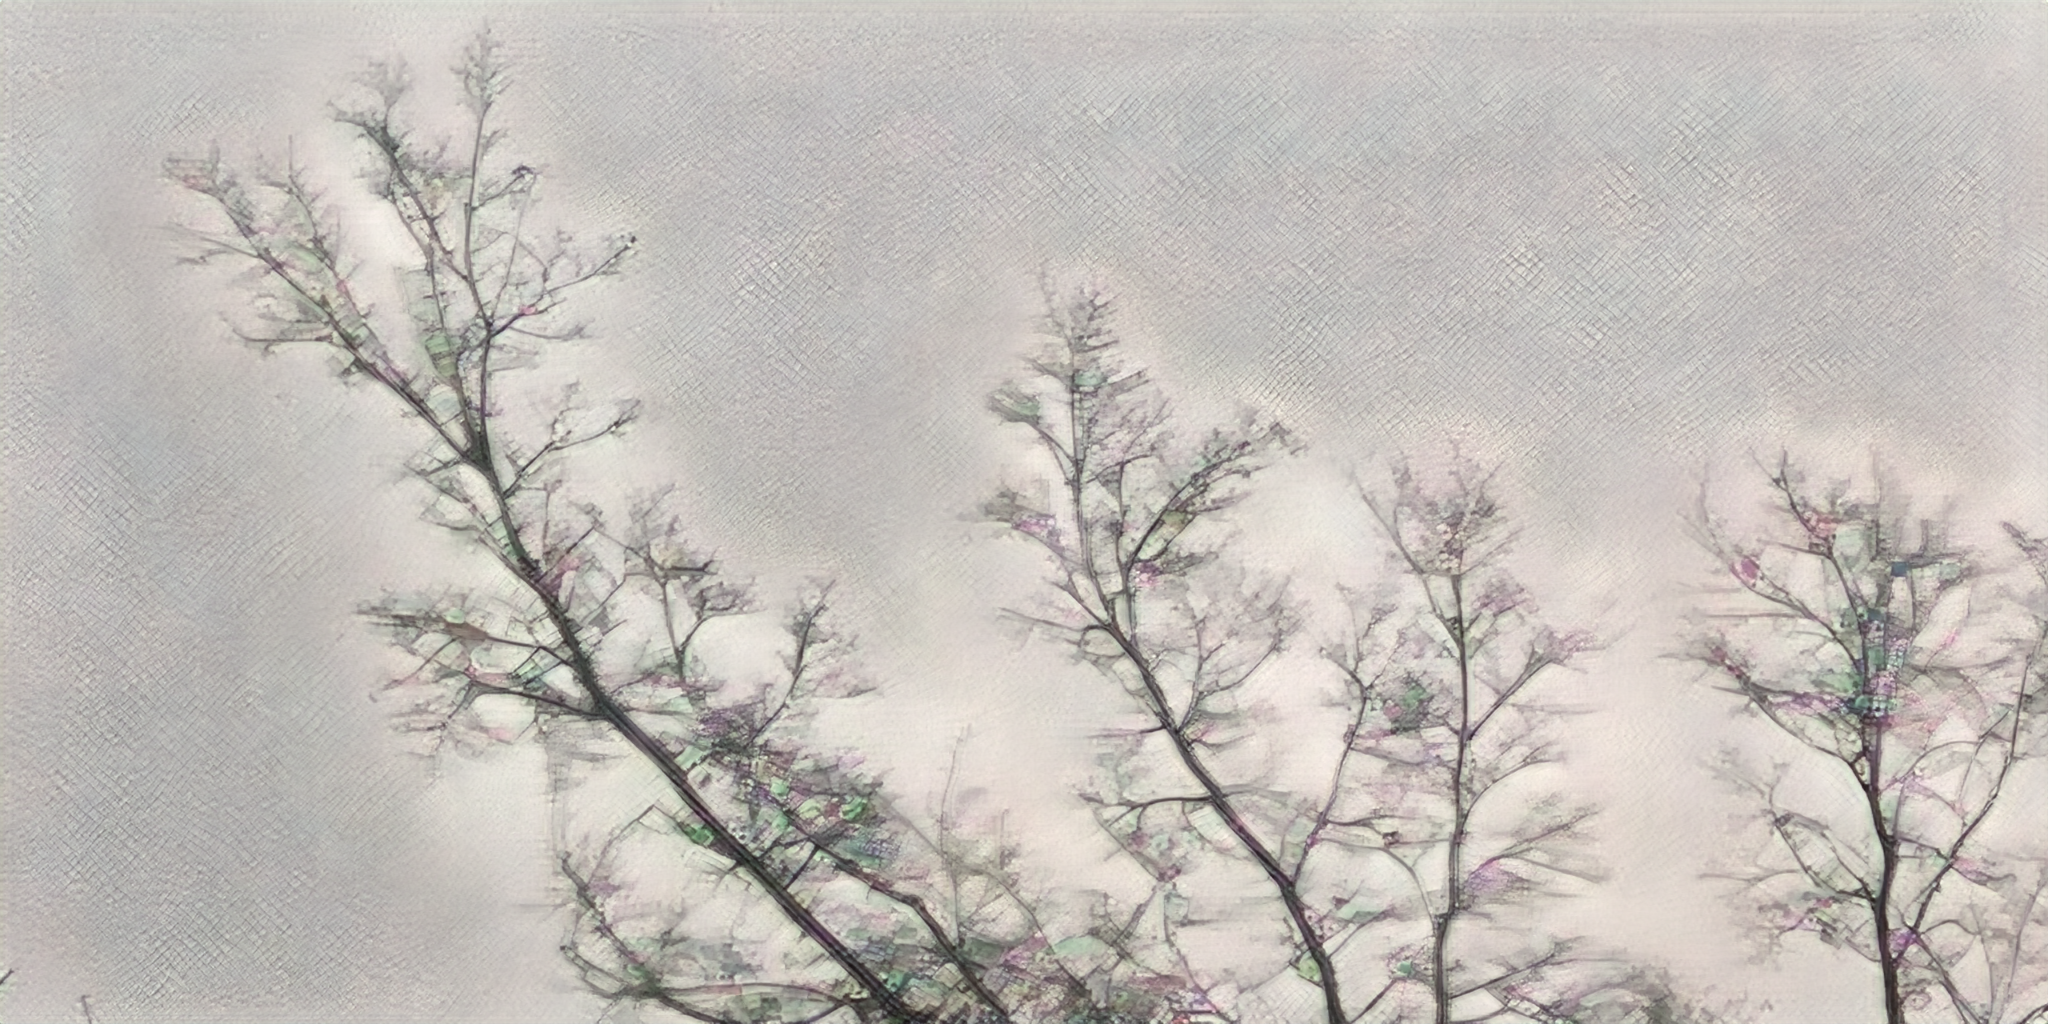
\includegraphics[height=2cm]{pic/pic0201a.png}}
        
        \subfloat[pretrain]{\label{fig:0201b}
        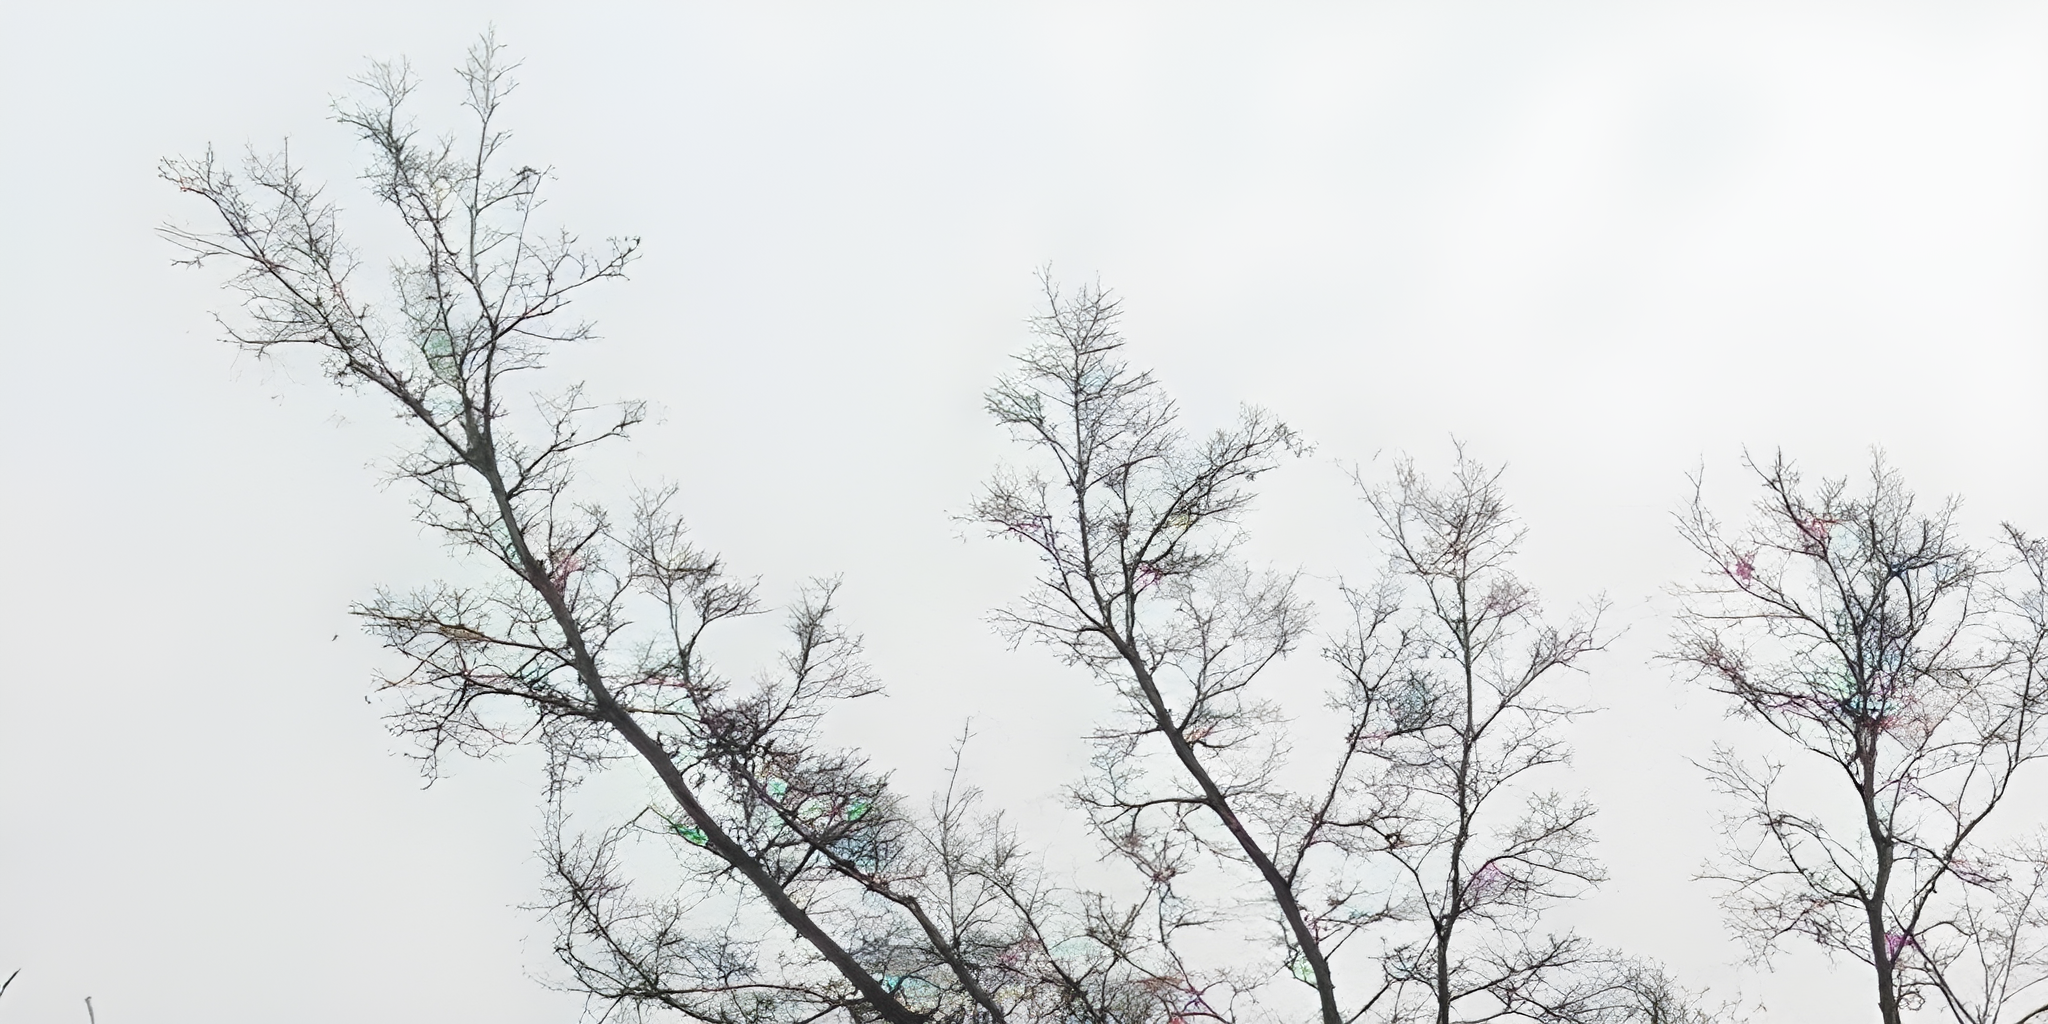
\includegraphics[height=2cm]{pic/pic0201b.png}}
        \caption{相机影像对比}
        \label{fig:0201}
    \end{figure}
\end{frame}

\begin{frame}{影像集}
    以realESRGAN为例, 使用动漫图片和遥感影像, 分别使用预训练和finetune后的模型进行对比

    \begin{figure}[!htbp]
        \centering
        \subfloat[finetune]{\label{fig:0201a}
        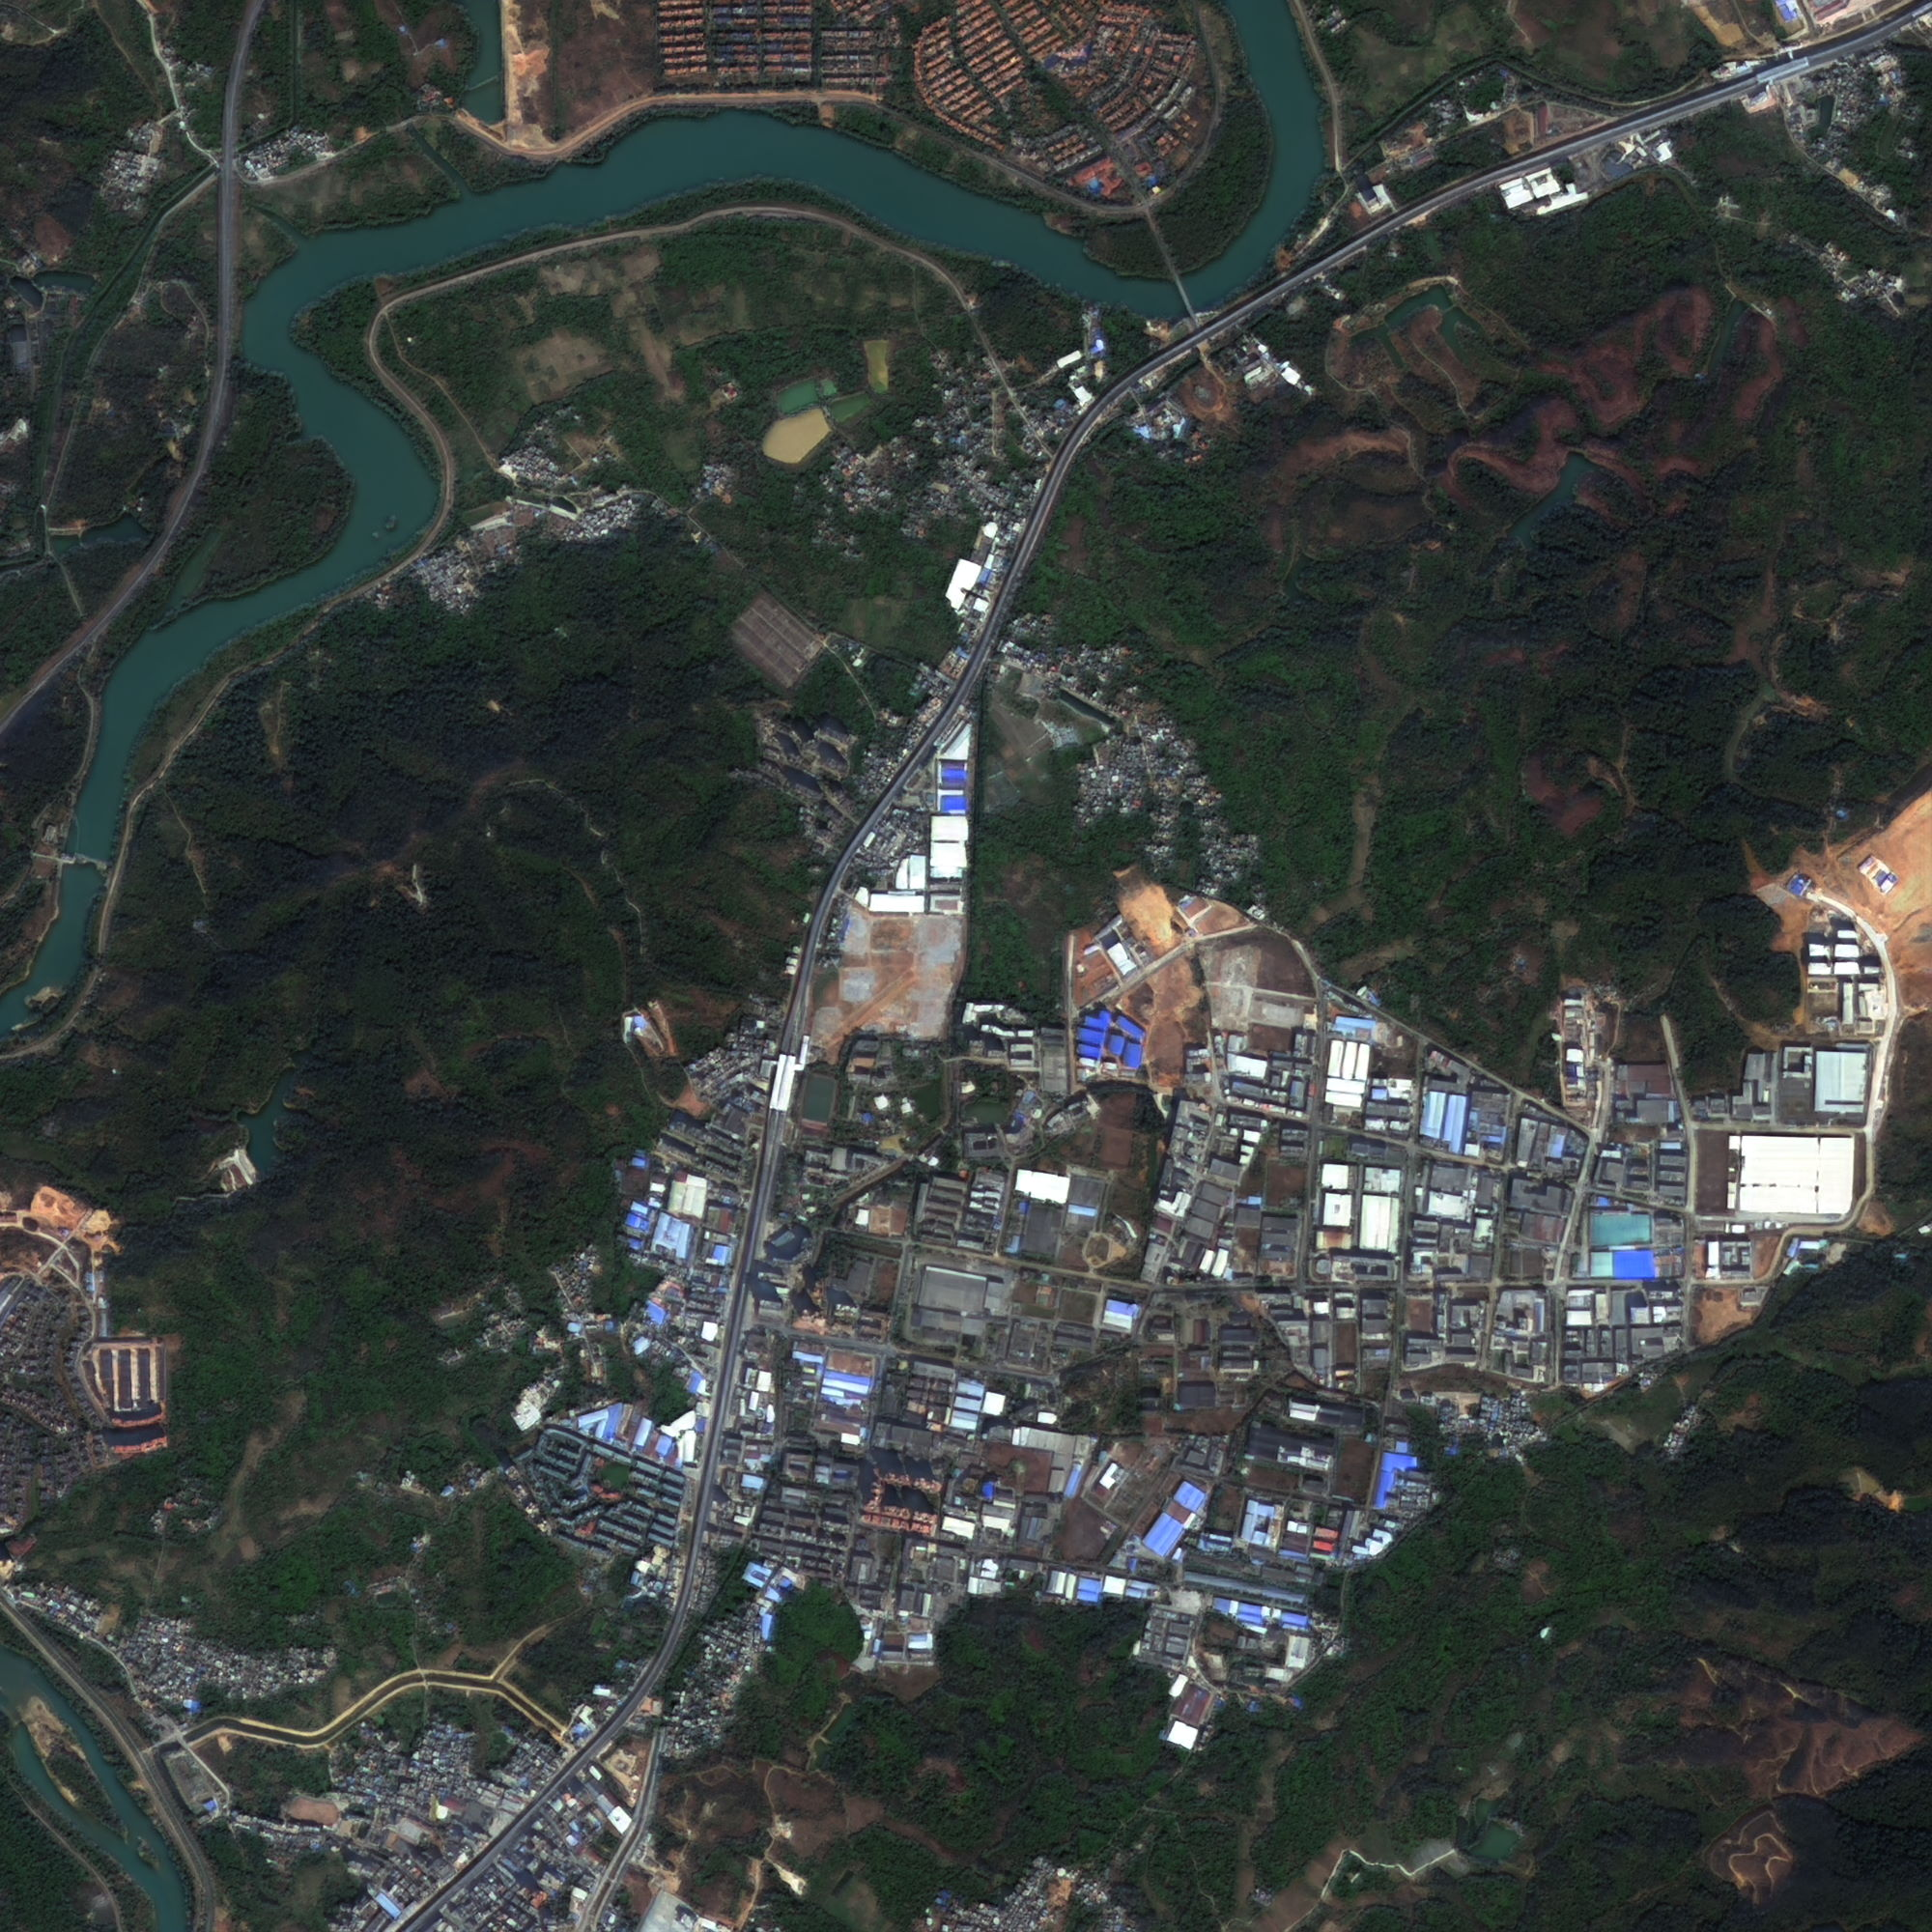
\includegraphics[height=4cm]{pic/pic0202a.jpg}}
        \quad
        \subfloat[pretrain]{\label{fig:0201b}
        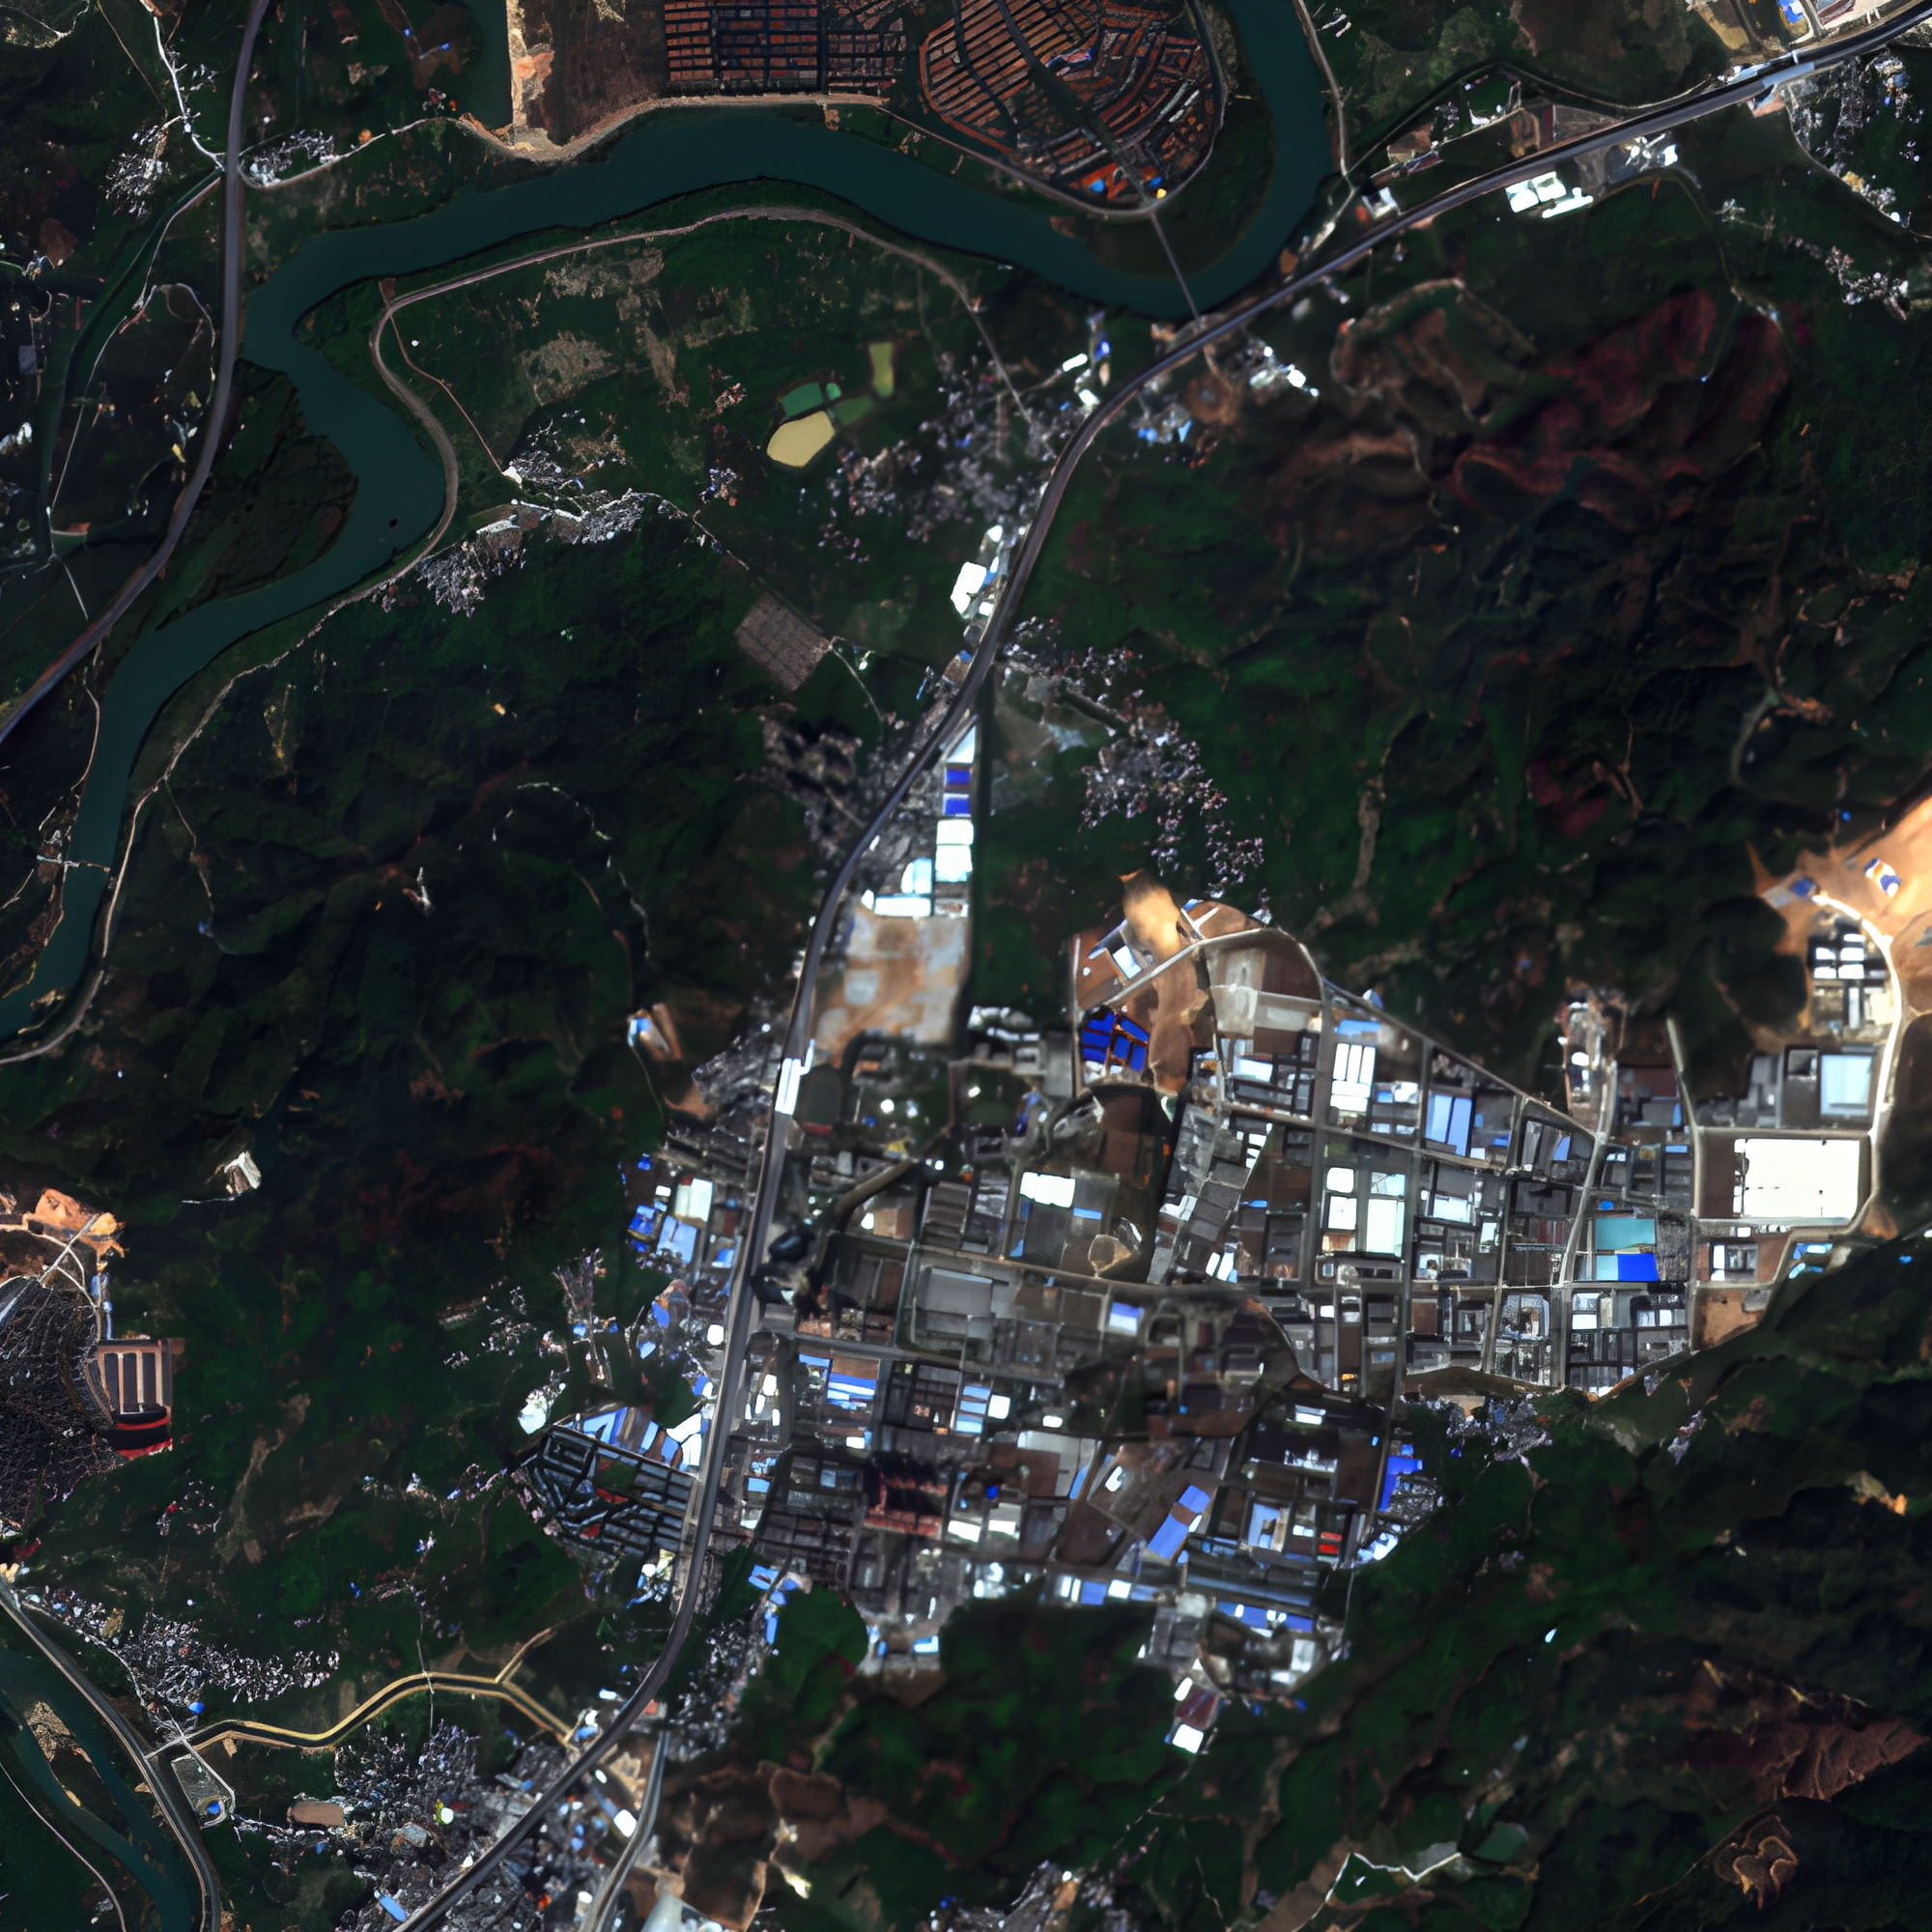
\includegraphics[height=4cm]{pic/pic0202b.jpg}}
        \caption{遥感图片对比}
        \label{fig:0202}
    \end{figure}

\end{frame}

\subsection{数据集与模型}
\begin{frame}{数据集}
    真实数据, DSGAN生成数据做对比

    不同模型之间的分析
\end{frame}
